\documentclass[12pt]{article} % Font size (can be 10pt, 11pt or 12pt) and paper size (remove a4paper for US letter paper)

\usepackage[fleqn]{amsmath}
\usepackage[fleqn]{mathtools}
\usepackage{graphicx} % Required for including pictures
\usepackage{wrapfig} % Allows in-line images
\usepackage{url}
\usepackage{mathpazo} % Use the Palatino font
\usepackage[T1]{fontenc} % Required for accented characters
\linespread{1.05} % Change line spacing here, Palatino benefits from a slight increase by default
\usepackage{csquotes}

\makeatletter
\renewcommand\@biblabel[1]{\textbf{#1.}} % Change the square brackets for each bibliography item from '[1]' to '1.'
\renewcommand{\@listI}{\itemsep=0pt} % Reduce the space between items in the itemize and enumerate environments and the bibliography

\renewcommand{\maketitle}{ % Customize the title - do not edit title and author name here, see the TITLE block below
	\begin{center} % Right align
		{\LARGE\@title} % Increase the font size of the title
		
		\vspace{15pt} % Some vertical space between the title and author name
		{\large\@author} % Author name
		\\\@date % Date
		
	\end{center}
}
\usepackage[margin=0.7in]{geometry}
\usepackage{xcolor}
\usepackage{textcomp}
\definecolor{dkgreen}{rgb}{0,0.6,0}
\definecolor{gray}{rgb}{0.5,0.5,0.5}
\definecolor{mauve}{rgb}{0.58,0,0.82}

\usepackage{listings}
\lstset{
	frame=single,
	breaklines=true,
	postbreak=\raisebox{0ex}[0ex][0ex]{\ensuremath{\color{red}\hookrightarrow\space}}
}
\lstnewenvironment{C}
{\lstset{frame=tb,
		language= C, 
		aboveskip=3mm,
		belowskip=3mm,
		showstringspaces=false,
		columns=flexible,
		basicstyle={\small\ttfamily},
		numbers=none,
		numberstyle=\tiny\color{gray},
		keywordstyle=\color{blue},
		commentstyle=\color{dkgreen},
		stringstyle=\color{mauve},
		breaklines=true,
		breakatwhitespace=true
		tabsize=3
	}
} {}

\title{Project 4 Report}
\author{Vedanth Narayanan}
\date{\today}

\begin{document}
	\maketitle
	\section*{Questions}
	\begin{enumerate}
		\item \textbf{What your own-choice quantity was and how it fit into the simulation.}\\
		For my choice quantity, I chose to introduce bears. Initially, I didn't think about this too  much and even considered it being boring, however it turned out to be really interesting. Bears are omnivores, so I thought it would be interesting for them to be having an effect on both grains and deers. Although bears do not eat particularly eat grains in real life, they do for the purposes of this simulation.\\
		The thing that made this interesting was that I made sure to add some particular new rules, and modified some existing rules. Since bears were going to eat grains as well, the grain growth was increased to 12.5. The amount of grains that a deer eats was increased to 0.7. I treated what the bear eats as a ratio. The bear eats 0.7 deers every month, and 0.3 grains every month. You can infer here that the bears definitely like eating the deer more than the grains, similar to how toddlers prefer eating everything else to broccoli. The temperature and precipitation were altered only slightly so they produced before results for the graph. The details of weather are negligible.\\
		Getting the grain heights was fairly methodical. We already know that the grains grow depending on the temperature and precipitation factors. The height goes down based on how much is eaten by both deers and bears.\\
		The logic for the deer worked in a manner where the deer population went up based on the ratio of grain height to deer. With a ratio between 0-1, deer population went down. Based on how many bears existed, and the how much they collectively ate, the deer population once again went down.\\
		The bears' logic was simple. Unlike for the grains and deer, the bear population is significantly only affected by the deer population. As a reminder, there is an interesting distinction here. Although the bears eat both deer and grains, the population is \emph{only} affected by the number of deers that exist. Based on the deer-to-bear ratio, the population went up. When the ratio dropped to less than 0.5, the population went down.
		\item \textbf{A table showing values for temperature, precipitation, number of graindeer, height of the grain, and your own-choice quantity as a function of month number.}
		\begin{center}
			\begin{tabular}{ | l | l | l | l | l | l | } \hline
				Month & Temp & Precip & Grains & Deers & Bears \\ \hline
				0 & 1.22 & 8.52 & 0 & 3 & 3 \\ \hline
				1 & 3.87 & 16.04 & 0 & 1 & 3 \\ \hline
				2 & 10.5 & 11.91 & 10 & 2 & 1 \\ \hline
				3 & 11.7 & 17.71 & 18 & 5 & 2 \\ \hline
				4 & 16.67 & 13.56 & 16 & 7 & 3 \\ \hline
				5 & 21.6 & 10.9 & 10 & 8 & 4 \\ \hline
				6 & 20.6 & 5.78 & 3 & 5 & 5 \\ \hline
				7 & 22.66 & 6.46 & 0 & 1 & 5 \\ \hline
				8 & 14.37 & 2.47 & 4 & 1 & 3 \\ \hline
				9 & 3.65 & 1.35 & 5 & 2 & 1 \\ \hline
				10 & -2.94 & 0 & 3 & 5 & 2 \\ \hline
				11 & -5.03 & 8.74 & 0 & 3 & 3 \\ \hline
				12 & -4.86 & 8.59 & 0 & 1 & 3 \\ \hline
				13 & -1.93 & 9.02 & 0 & 1 & 1 \\ \hline
				14 & 11.27 & 12.12 & 10 & 4 & 1 \\ \hline
				15 & 13.28 & 18.43 & 14 & 7 & 3 \\ \hline
				16 & 19.64 & 10.94 & 8 & 7 & 4 \\ \hline
				17 & 23.03 & 9.84 & 1 & 4 & 4 \\ \hline
				18 & 21.75 & 10.45 & 0 & 1 & 4 \\ \hline
				19 & 16.8 & 4.99 & 0 & 1 & 2 \\ \hline
				20 & 13.4 & 3 & 7 & 3 & 1 \\ \hline
				21 & 5.95 & 4.24 & 11 & 6 & 3 \\ \hline
				22 & -0.56 & 0.73 & 6 & 6 & 4 \\ \hline
				23 & 0.93 & 9.91 & 1 & 3 & 4 \\ \hline
				24 & -5.63 & 14.16 & 0 & 1 & 2 \\ \hline
				25 & 1.59 & 8.80 & 0 & 1 & 1 \\ \hline
				26 & 4.09 & 16.64 & 2 & 4 & 1 \\ \hline
				27 & 16.63 & 13.45 & 1 & 3 & 3 \\ \hline
				28 & 14.77 & 8.13 & 3 & 3 & 3 \\ \hline
				29 & 21.43 & 5.15 & 0 & 1 & 3 \\ \hline
				30 & 19.48 & 10.43 & 0 & 1 & 1 \\ \hline
				31 & 22.22 & 5.8 & 0 & 1 & 1 \\ \hline			
				32 & 11.09 & 0.66 & 10 & 4 & 1 \\ \hline
				33 & 5.73 & 2.9 & 13 & 7 & 3 \\ \hline
				34 & 1.47 & 3.94 & 8 & 7 & 4 \\ \hline
				35 & -1.52 & 0.97 & 2 & 4 & 4 \\ \hline
				36 & -2.36 & 13.98 & 0 & 1 & 4 \\ \hline
			\end{tabular}
		\end{center}			
		\begin{center}
			\begin{tabular}{ | l | l | l | l | l | l | } \hline
				Month & Temp & Precip & Grains & Deers & Bears \\ \hline
				37 & 5.19 & 15.25 & 3 & 2 & 2 \\ \hline
				38 & 4.92 & 17.39 & 5 & 4 & 2 \\ \hline
				39 & 14.41 & 13.5 & 7 & 6 & 3 \\ \hline
				40 & 20.30 & 9.61 & 2 & 3 & 4 \\ \hline
				41 & 21.27 & 13.45 & 0 & 1 & 2 \\ \hline
				42 & 24.73 & 3.92 & 0 & 1 & 1 \\ \hline
				43 & 16.23 & 6.23 & 2 & 4 & 1 \\ \hline
				44 & 11.83 & 2.16 & 9 & 7 & 3 \\ \hline
				45 & 10.89 & 1.15 & 14 & 8 & 4 \\ \hline
				46 & 2.76 & 5.88 & 9 & 8 & 5 \\ \hline
				47 & -2.34 & 9.96 & 1 & 4 & 5 \\ \hline
				48 & -2.71 & 12.79 & 0 & 1 & 3 \\ \hline
				49 & 3 & 17.18 & 0 & 1 & 1 \\ \hline
				50 & 6.68 & 12.09 & 7 & 4 & 1 \\ \hline
				51 & 17.17 & 19.25 & 5 & 7 & 3 \\ \hline
				52 & 15.51 & 16.88 & 3 & 4 & 4 \\ \hline
				53 & 23.06 & 8.9 & 0 & 1 & 4 \\ \hline
				54 & 22.87 & 3.42 & 0 & 1 & 2 \\ \hline
				55 & 21.18 & 0.28 & 0 & 1 & 1 \\ \hline
				56 & 12.69 & 0 & 8 & 4 & 1 \\ \hline
				57 & 4.05 & 0 & 8 & 7 & 3 \\ \hline
				58 & 1.86 & 1.38 & 3 & 4 & 4 \\ \hline
				59 & -4.74 & 9.77 & 0 & 1 & 4 \\ \hline
				60 & -5.33 & 5.79 & 0 & 1 & 2 \\ \hline
				61 & 1.32 & 15.65 & 0 & 1 & 1 \\ \hline
				62 & 11.15 & 19.39 & 8 & 4 & 1 \\ \hline
				63 & 14.8 & 13.79 & 10 & 7 & 3 \\ \hline
				64 & 20.86 & 11.67 & 4 & 4 & 4 \\ \hline
				65 & 19.98 & 6.87 & 0 & 1 & 4 \\ \hline
				66 & 22.56 & 3.05 & 0 & 1 & 2 \\ \hline
				67 & 15.55 & 4.59 & 3 & 3 & 1 \\ \hline
				68 & 9.83 & 3.24 & 12 & 6 & 3 \\ \hline
				69 & 3.85 & 2.75 & 10 & 7 & 4 \\ \hline
				70 & -2.42 & 6.8 & 3 & 4 & 4 \\ \hline
				71 & -5.78 & 5.87 & 0 & 1 & 4 \\ \hline
			\end{tabular}
		\end{center}
		\item \textbf{A graph showing temperature, precipitation, number of graindeer, height of the grain, and your own-choice quantity as a function of month number.} \\
		The x-axis, Time, starts January 2016 and goes through December of 2021. Every number essentially has a particular number assigned to it. The y-axis title is vague, because it involves a variety of units. Deer and bear are just populations. Temperature and precipitation are in Celsius and cm, respectively. Grain heights aren't specified at all, however, they seem to make more sense in inches.\\
		\hspace*{-2.7cm}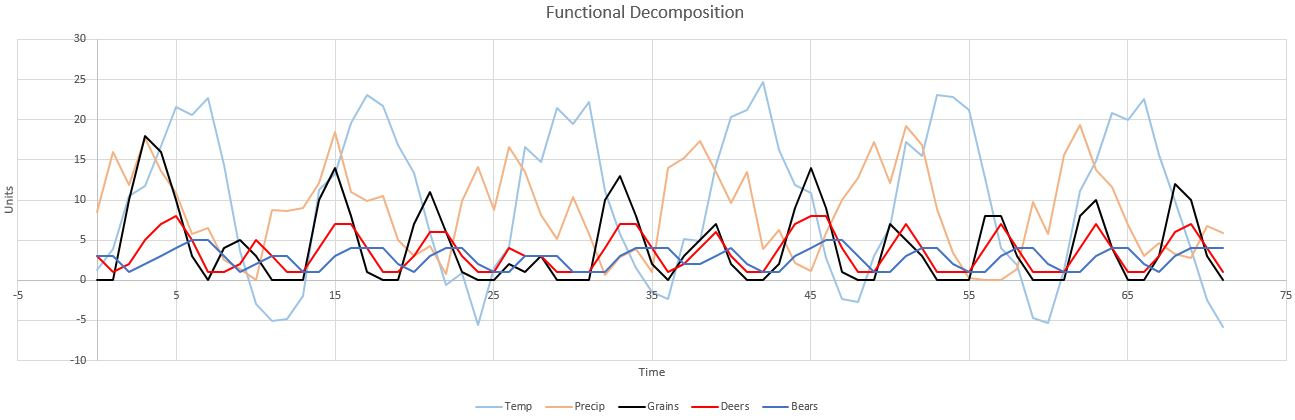
\includegraphics[scale=0.65]{graph}
		
		\item \textbf{A commentary about the patterns in the graph and why they turned out that way.}\\
		Before getting into the details it's good to mention that there were more than a handful of tests that were run to find the right numbers. This is one of the reasons why you'll notice the modified variables mentioned in question 1. That being said, the patterns in the graph are very much prominent. As a little note, the temperature and precipitation are lighter colored, so the viewer can focus more on the grain, deer, and bear growth.\\
		For the most part, when the temperature and/or precipitation goes up, we see the grain spikes up as well. When the temperature and/or precipitation go down, the grain growth also follow suit. Depending on the grain growth, we can see trends with both the deers and bears. The distinction to keep in mind is the bear growth dictated by the deer growth, and is not directly influenced by the grain growth.\\
		When the grain growth goes up, the deer population clearly increases, and this can be noticed in any of the major spikes. The bear population also increases, but most of the time does not surpass the deer population. This just happens to be because of the way the logic was implemented. When the grain height goes down, the deer population quickly diminishes, but this is not entirely the case for the bears. When bears are not eating deers, they survive off grains before going down. This can be noticed in a couple places, like around x=20, or past x=45.\\
		There are places where the grain height is pretty high, and the deer or bear population does not seem to increase significantly. Note that this was only because the logic was for the population growth was not the best it could be. 
	\end{enumerate}
\end{document}
